\documentclass{scrreprt} % comment this out when done editing
% \documentclass{standalone}
% \usepackage{standalone}
\usepackage{chez}

\begin{document}

\section{Unit 02}

\subsection{September 02, 2021 - Vectors}

\begin{remark}
Let's suppose we have a vector $A$ of length $2$ meters and $40^{\circ}$ N of E

We also have a vector $B$ of lf length $2m$ and $8^\circ$ W of S

We wish to compute $A + B$

Graph A:

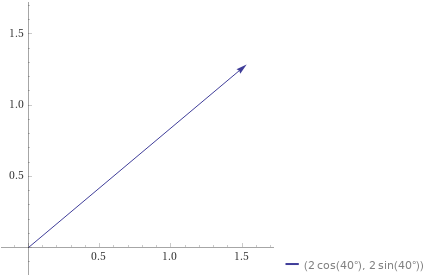
\includegraphics[width=250px]{2021-09-02-09-01-20.png}

Graph B:

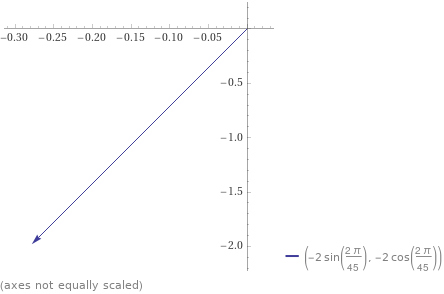
\includegraphics[width = 250px]{2021-09-02-09-04-43.png}

Let's convert vectors to $x$ and $y$ coordinates, then

$$A = \begin{bmatrix}1.53209\\1.28558\end{bmatrix},
  B = \begin{bmatrix}-0.273846\\-1.98054\end{bmatrix}$$

Then, $$A + B = \begin{bmatrix}1.53209+(-0.273846)\\1.28558+(-1.98054)\end{bmatrix}
              = \begin{bmatrix}1.25374\\-0.694956\end{bmatrix}
              = 1.25374\hat{i} - 0.694956\hat{j]}$$

To find the length, we can use the Pythagorean theorem:

$$1.25374^2 + (-0.694956)^2 = 1.43347$$

\end{remark}

\begin{definition}[Unit Vectors]
  \begin{itemize}
    \item $\hat{i}$ is the unit vector in the $x$ direction
    \item $\hat{j}$ is the unit vector in the $y$ direction
    \item $\hat{k}$ is the unit vector in the $z$ direction
  \end{itemize}
\end{definition}

\begin{remark}
  The syntax for a vector in the TI-89 graphing calculator is 
  $[r,\angle \theta $. 

  \begin{itemize}
    \item You can also switch between polar (cylindrical) and rectangular.
  \end{itemize}
\end{remark}

\begin{remark}
  You can take the derivative of a vector with respect to each of its components.
\end{remark}

\end{document}